\section{雲}

系外惑星・褐色矮星大気の推定では、雲のモデルが必要である観測スペクトルも多い。雲のモデルは、実際の解析には簡単に灰色の色依存性のない連続オパシティとして扱われることも多い。しかしここでは雲の微物理に踏み込んだモデルを紹介する\footnote{雲の微物理の深い議論はPruppacher and Klett\cite{pruppacher2010microstructure}を参照}。特に系外惑星の雲モデルのseminal paperであるAckerman and Marley\cite{ackerman2001precipitating}に雲モデルを紹介する。 雲は、大気中に存在する気体から固体もしくは液体に想定することで発生する。地球大気の雲は主にH2Oによるものであるが、液体の雲(水雲)と固体の雲(氷雲)がある。 表\ref{tab:input2}に、系外惑星や褐色矮星で考える主な雲の構成成分を示した。

\begin{table}[!tbh]
\begin{center}
\caption{典型的な雲粒子の構成成分とその物質密度。\label{tab:input2}}
\begin{tabular}{lcc}
  \hline\hline
  通称&分子式&物質密度$\delta_\cond (\mathrm{g/cm^{3}}$) \\
  \hline
water&H2O& 1 \\
&NH3& \\
Fe (固体) &Fe&7.875\\
ferrous oxide&FeO&5.987\\
phosphate &H3PO4& \\
&KCl&\\
&Na2S&\\
&TiO&\\
&SiC&\\
&VO&\\
hematite     &Fe2O3&5.275\\
magnetite    &Fe3O4&5.200\\
fayalite     &FeSiO4&4.393\\
corundum     &Al2O3&3.987\\
quartz       &SiO2&2.648\\
rutile       &TiO2&4.245\\
enstatite    &MgSiO3&3.194\\
forstelite   &Mg2SiO4&3.214\\
\end{tabular}
\end{center}
\end{table}

\subsection*{雲粒子の終端速度}\label{ss:termv}

雲粒子が落下し、空気抵抗力$F_d$+浮力$F_a$と重力が釣り合った定常の速度になったとする。この速度を終端速度(terminal velocity)という。釣り合いの式は
\begin{align}
F_d + F_a = m (r) g 
\end{align}
である。$m(r)$は雲粒子の質量、$g$は重力定数である。雲粒子の物質密度を$\delta_\cond$、大気の密度を$\rho$とする。
\begin{align}
m(r) &= \frac{4 \pi}{3} r^3 \delta_\cond \\
F_a &= \frac{4 \pi}{3} r^3 \rho g 
\end{align}
なので
\begin{align}
\label{eq:Fd}
F_d &= \frac{4 \pi}{3} r^3 (\delta_\cond - \rho) g \\
&\approx  \frac{4 \pi}{3} r^3 \delta_\cond g 
\end{align}
となる。最後の近似は、通常$\delta_\cond \gg \rho$なので浮力を無視している場合である。

抵抗力$F_d$は、一般的に終端速度$v_f$と抵抗係数$C_d$を用いて
\begin{align}
F_d = C_d \frac{\rho v_f^2}{2} (\pi r^2)  
\end{align}
の形にかける(証明略)。ここで無次元数レイノルズ数
\begin{align}
\label{eq:Reynolds}
N_{re} = \frac{2 \rho v_f r}{\eta}
\end{align}
を用いて、
\begin{align}
F_d = 6 \pi \eta r v_f \left( \frac{C_d N_{re}}{24} \right)
\end{align}
の形に書き直せる。式(\ref{eq:Fd})と合わせると
\begin{align}
\label{eq:gcloud}
v_f(r) = \frac{2}{9 \eta}  g r^2 (\delta_\cond - \rho) \left( \frac{C_d N_{re}}{24} \right)^{-1}
\end{align}
となる。ただし$\eta$はdynamic viscosity.


ここで$C_d$はレイノルズ数によってことなる。$N_{re} \ll 1$の場合、
\begin{align}
C_d = \frac{24}{N_{re}}
\end{align}
のStokes flowとなる。粒子サイズが小さい場合、粒子表面での滑りが生じ、そのための補正、Cunningham補正係数$(1+1.26 N_{Kn})$、$N_{Kn}=k_B T/\sqrt{2 \pi r^2 P L}$はKnudsen数の補正をいれる。
結果の終端速度は
\begin{align}
\label{eq:sfcloud}
v_f^{sf}(r) = \frac{2}{9 \eta} g r^2 (\delta_\cond - \rho) (1+1.26 N_{Kn})
\end{align}
となり粒径$r$の二乗に比例する。大きいレイノルズ数ではこのような近似はできないが、
$N_{re} = 0.01-300$くらいの場合は、$v_f$が$r$に、$N_{re} > 300$の場合は$r^{1/2}$にだいたい比例することが知られている

dynamic viscosity についてはRosnerの教科書 \cite{rosner2012transport}により
\begin{align}
\label{eq:dyvis}
\eta = \frac{5}{16} \frac{\sqrt{\pi m k_B T}}{\pi d^2} \frac{(k_B T/\varepsilon)^{0.16}}{1.22}
\end{align}
で与えられる。Rosnerの教科書 \cite{rosner2012transport}には、さまざまな大気成分について分子直径$d$、Lennard-Jones potentialと$k_B$の比が与えられている。

中レイノルズ数では、無次元数であるデービス数(Davies number)\footnote{Best numberとも。}$N_D = C_d N_{re}^2 $を考える。式(\ref{eq:gcloud})にレイノルズ数の定義(\ref{eq:Reynolds})から$v_f$を消去することで、
\begin{align}
\label{eq:davies}
N_D = C_d N_{re}^2 = \frac{32}{3 \eta^2} g r^3 \rho (\delta_\cond - \rho)
\end{align}
を求めることができる。

これと$x=\log{N_D}$と$y=\log{N_{re}}$の関係式($y=f(x)$)を実測値からフィットしたものを用いることで、$N_{re}$を求め、レイノルズ数の定義(\ref{eq:Reynolds}式より、
\begin{align}
\label{eq:vfmid}
v_f = \frac{\eta}{2 \rho r} e^{f(\log{N_D})}
\end{align}
と終端速度が求まる。

Pruppacher and Klett\cite{pruppacher2010microstructure}のTable 10.1の値を用いると、
\begin{align}
\label{eq:daviesn}
f(x) = -0.0088 x^2+0.85 x -2.49
\end{align}
がよくフィットする(図\ref{fig:davies})。
また$N_{re}>500$では、Ackerman and Marley (2001) \cite{ackerman2001precipitating}に従い、$C_d=0.45$を採用するとする。
\begin{align}
\label{eq:vflarge}
v_f = \frac{\eta}{2 \rho r} \sqrt{\frac{N_D}{C_d}}
\end{align}
となる。

\begin{figure}[htb]
\begin{center}
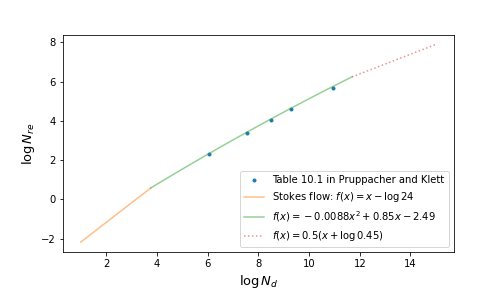
\includegraphics[width=\linewidth]{fig/clouds/davies_reynolds.png}
\caption{デービス数・レイノルズ数の関係.\label{fig:davies}}
\end{center}
\end{figure}

以上をまとめると
\begin{align}
\label{eq:vterm}
v_f =
\begin{cases}
&\displaystyle{\frac{2}{9 \eta} g r^2 (\delta_\cond - \rho) (1+1.26 N_{Kn}) } \nonumber \\
&\,\,\,\,\, \mbox{\, for $N_D < 42$ ($N_{re} < 2$)} \\
&\displaystyle{ \frac{\eta}{2 \rho r} \exp{(-0.0088 \log^2{N_D}+0.85 \log{N_D} -2.49)}} \nonumber \\
&\,\,\,\,\, \mbox{\, for $42 \le N_D < 10^5$ ($2 \le N_{re} < 500$)} \\
&\displaystyle{\frac{\eta}{2 \rho r} \sqrt{\frac{N_D}{C_d}}} \nonumber \\
&\,\,\,\,\, \mbox{\, for $10^5 \ge N_D$ ($500 \ge N_{re}$)} 
\end{cases}
\end{align}
となる。境界条件は接続するようにとっている。

\begin{figure}[htb]
\begin{center}
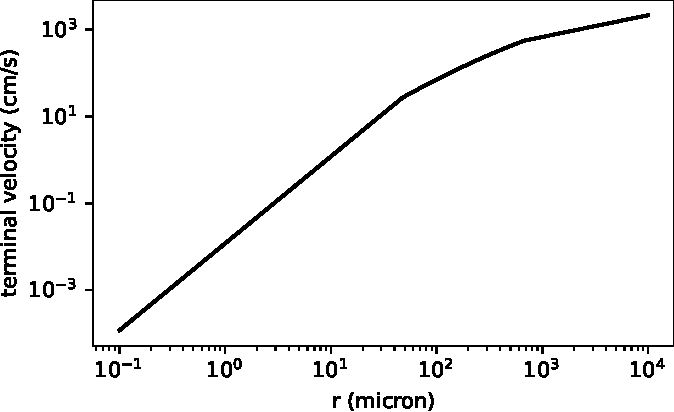
\includegraphics[width=\linewidth]{fig/clouds/vterm.pdf}
\caption{雲粒子半径と終端速度。地球大気・地球重力、$T=300$Kの場合。\label{fig:vterm}}
\end{center}
\end{figure}


\begin{itembox}{問題}
人間の会話や呼吸で排出される水について考えよう。WHOの定義では直径5\textmu m以上のの水滴をdroplet(飛沫)、直径5\textmu m以下の半径の水滴をaerosol(エアロゾル)あるいはdroplet nuclei(飛沫核)と定義している。地面から1.5mのところにある口から排出された直径5 \textmu mのエアロゾルは、何分くらい空気中に滞留するか?ここでは空気の流れはなく、水滴の蒸発もないとする。
\end{itembox}







\subsection*{蒸気圧曲線と雲底面}

単一成分の気体-固体、気体-液体の相変化による雲を考える。雲はある高度以上で気体が固体または液体に相変化することで発生する。雲の生成・消滅は複雑な物理によるが、ここでは蒸気圧曲線と分圧が一致した高さを雲底を簡単に定義する。すなわち気体成分の体積混合率を$\xi_v(P)$とすると
\begin{align}
P(T) = P_\mathrm{sat}(T)/\xi_v(P)
\end{align}
となる$(P,T)$が雲底であるとする(図\ref{fig:pbase})。また蒸気圧$P_\mathrm{sat}(T)$はClausius-Clapeyronの式から潜熱$l$を用いて
\begin{align}
P_\mathrm{sat}(T) = P_\mathrm{sat,0} e^{-l/RT}
\end{align}
の形で書ける(系外惑星探査6.2.3 p153)。


複数成分の気体からなる雲の場合、"気体成分"の体積混合比$\xi_v(P)$をどのように求めるかという問題もある。化学平衡計算をして求めるか、もしくは作れる最大の量を作るという考えかたもある。後者の場合、たとえばエンスタタイト($\mathrm{Mg Si O_3}$)であれば、それぞれの元素の体積混合比からの律速量を利用して
\begin{align}
\xi_v = \mathrm{min} [ \xi(\mathrm{Mg}),\xi(\mathrm{Si}),\xi(\mathrm{O})/3 ]
\end{align}
となる。

%Ackerman and Marley cloud model.ipynb (exojax)
\begin{figure}[htb]
\begin{center}
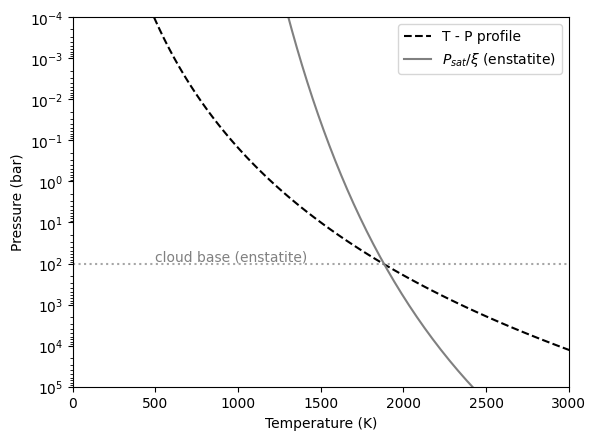
\includegraphics[width=\linewidth]{fig/clouds/pbase.pdf}
\caption{雲底の決め方。温度圧力プロファイルと蒸気圧曲線を体積混合率で割ったものとの交点が雲底となる。\label{fig:pbase}}
\end{center}
\end{figure}

\subsection*{Ackerman and Marleyの雲分布モデル}


系外惑星や褐色矮星の雲のモデルとしてよく用いられるAckerman \& Marley (2001)\cite{ackerman2001precipitating}(AM01)に基づき、いくつか修正して解説したい。
簡単のためある分子が凝縮して雲になることを考える。例えば水による雲は大気中では気体の状態($\vapor$)と雲の状態($\cond$)の二種類をとる。二つの状態の総和を$\total$で表す。混合比は混乱を避けるため体積混合比\footnote{体積混合比、すなわち数混合比では、一個をどう数えるか定義しなくてはならない。例えば、雲全体が含む分子の個数の場合もあれば、それぞれ大きさの違う(つまり含む分子の個数が異なる)雲粒子の個数の総和を想定する場合もありうる。}ではなく質量混合比で考える。
全質量混合比$X_\total (z) $は、雲の質量混合比$X_\cond$とガスの質量混合比$X_\vapor (z)$の和である。
\begin{align}
%\xi_m_\total (z) = \xi_m_\cond (z) + \xi_m_\vapor (z)
X_\total (z) = X_\cond (z) + X_\vapor (z)
\end{align}

このモデルではまず、代表サイズの雲粒子を考え、鉛直方向の輸送と降雨による凝縮体の沈降のバランス
\begin{align}
\label{eq:AM01}
%- \Kzz \frac{\partial}{\partial z} {\xi_m_\total (z)} - \overline{v}_f (z) \xi_m_\cond (z) = 0
- \Kzz \frac{\partial}{\partial z} {X_\total (z)} - \overline{v}_f (z) X_\cond (z) = 0
\end{align}
が基本的な式となる。ここに$\Kzz(z)$は鉛直方向の渦拡散係数(単位は$\mathrm{cm^2/s}$)、$\overline{v}_f(z)$は 雲粒子の典型的沈降速度である。


式(\ref{eq:AM01})を解くためには、$X$の三状態についてもう一つ拘束条件が必要である。ここでは
\begin{align}
%\xi_m_\cond (z)/\xi_m_\total (z) = \mathrm{const.} \equiv k_c
X_\cond (z)/X_\total (z) = \mathrm{const.} \equiv k_c
\end{align}
と仮定しよう。すると微分方程式(\ref{eq:AM01})は
\begin{align}
\label{eq:AM01c}
\frac{\partial}{\partial z} {X_\cond (z)} = - \frac{ k_c \overline{v}_f (z)}{\Kzz(z)} X_\cond (z) 
\end{align}
となる。

式(\ref{eq:AM01c})をみると$\overline{v}_f (z) \propto \Kzz(z)$と仮定できれば、この微分方程式は簡単に解けることがわかる。AM01ではそのような仮定を課しているようだ。つまり、沈降速度$\overline{v}_f(z)$が鉛直渦の速度スケール$v_\mathrm{eddy}(z) = \Kzz(z)/L$、ここに$L$は対流の典型的スケールに比例するとし、ここでは定数であるとする\footnote{AM01ではこれを定数としない定式化もなされている。定数としたものをHeuristicな場合として提示されている。}。$\fsed$を定数として
\begin{align}
\overline{v}_f(z) = \fsed v_\mathrm{eddy}(z) = \fsed \Kzz(z)/L \mbox{\,\,\,\,($\fsed$仮定)}
\end{align}
と書けるという仮定を置く。この場合、雲底より上の解は
\begin{align}
\label{eq:AM01cx}
X_\cond (z) = X_\cond(0) \exp{\left( - \frac{ k_c \fsed}{L} z \right) }
\end{align}
となる。

$L=H(z=0)=H_0$と仮定し、$z$と$P$の関係が$H_0$の静水圧で決まると仮定すると式(\ref{eq:AM01cx})は
\begin{align}
X_\cond(P) = 
\begin{cases}
X_\cond(0) \left( \frac{P}{P_0} \right)^{f_{sed}/k_c} & P \le P_0 \\
0 & P > P_0
\end{cases}
\end{align} 
と書ける。ここに$P=P_0$は雲底の圧力である。
雲の混合率分布は図\ref{fig:vmrcloud}のような分布となる。

%Ackerman and Marley cloud model.ipynb (exojax)
\begin{figure}[htb]
\begin{center}
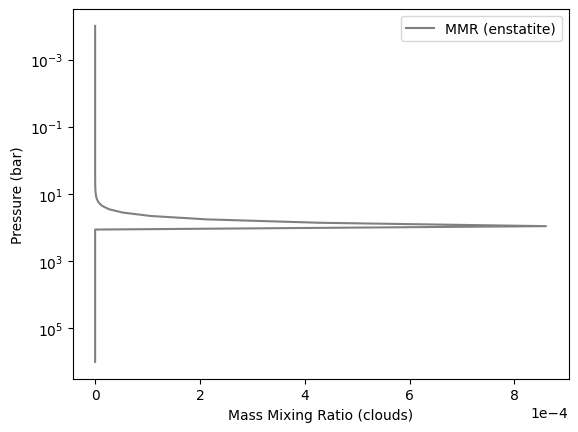
\includegraphics[width=\linewidth]{fig/clouds/mmrcloud.png}
\caption{雲の質量混合率の例。\label{fig:vmrcloud}}
\end{center}
\end{figure}

雲粒子のサイズ分布モデルを導入する。単位雲粒子半径あたりの雲の粒子数密度を
\begin{align}
    q(r) \equiv  \frac{d \mathcal{N}_\cond (r)}{d r} 
\end{align}
と定義する。ここに$\mathcal{N}_\cond(r)$は半径が$r$以下である粒子の数密度である。すなわち
\begin{align}
    \int_0^\infty q(r) dr = \int_0^\infty \frac{d \mathcal{N}_\cond (r)}{d r} dr = \mathcal{N}_\cond (\infty) \equiv N
\end{align}
が雲粒子の総数密度となる。ここでガスの数密度の表記である$n$と記号を変えている理由は、これは雲粒子の分子の数を数えているわけではないからであるという点に注意が必要である。雲粒子を構成する分子の数密度を$n_\cond$と表記すると、こちらは質量混合比と
\begin{align}
    X_\cond = \frac{\rho_\cond}{\rho} = \frac{\mu_\cond}{\mu} \frac{n_\cond}{n} 
\end{align}
の関係にある。${\mu_\cond}$は雲の構成分子の分子量である。ここに$\rho_\cond$は大気中で雲粒子全体が占める質量密度である($\mathrm{g/cm^3}$)。雲粒子自体の質量密度$\delta_\cond$と混同しないように注意が必要である(同じく単位は$\mathrm{g/cm^3}$)

また、$m_\cond$を雲粒子一つ一つの質量と定義すると、$dm_\cond/dr$が半径ごとの雲粒子の質量分布関数となる。雲粒子が球形であると仮定すると
\begin{align}
    \frac{dm_\cond}{dr} = \frac{4}{3} \pi r^3 \delta_\cond \frac{d \mathcal{N}_\cond (r)}{d r} = \frac{4}{3} \pi r^3 \delta_\cond q(r)
\end{align}
となる。

渦拡散係数と各粒子サイズ$r$における沈降速度$v_f(z; r)$が個別に与えられうるが、個別に与えた場合はこの「$\fsed$仮定」は一般にはなりたたない。

$\fsed$仮定を成り立たせるための一番強い仮定は各サイズに対して、
\begin{align}
v_f(z; r)= \fsed v_\mathrm{eddy}(z) = \fsed \Kzz(z)/L 
\end{align}
としてしまうことだが、これだと沈降速度のサイズ依存性を取り込めない。そもそも式(\ref{eq:AM01})は各粒子サイズに対して成り立つとしているわけではなく、なんらかの代表値でなりたつとしている。そこで$\fsed$仮定を代表操作に押し付けることになる。

いま沈降速度に対する代表操作を質量平均とする。すなわち
\begin{align} 
\label{eq:fsedw}
&\overline{v}_f(z) = \frac{\int v_f(m_\cond) dm_\cond}{M_c(z)} = \frac{\int_0^\infty v_f(z; r) (dm_\cond/dr) dr}{ \int_0^\infty (dm_\cond/dr) dr } \nonumber \\
&= \frac{\int_0^\infty dr \, v_f(z;r) r^3 q(r)}{ \int_0^\infty dr \, r^3 q(r)}
\end{align}
で対応付けられるとする。


高さ$z$の大気層において単位体積あたりの雲粒子の総質量は$M_c(z) = X_\cond(z) \rho $、ただし$\rho$は大気質量密度であることに注意。
%\begin{align} 
%M_c(z) 
%= \xi^c(z) m_c n_a = \xi^c(z) (\mu_\cond m_H) \frac{\rho}{\mu m_H}
%= \xi^c(z) (\mu_\cond/\mu) \rho = \epsilon \, \xi^c(z) \rho
%= X_\cond(z) \rho
%\end{align}
%$n_a$は大気全体の数密度、$m_c$は平均雲粒子質量、$m_H$は原子質量単位、$\mu_\cond$は雲粒子の平均分子量, $\mu$は大気全体の平均分子量、$\rho$は大気質量密度である。
%\begin{align} 
%\epsilon \equiv \mu_\cond/\mu
%\end{align}
%と定義した。
これが$\fsed$仮定を満たせばいいので
\begin{align} 
\label{eq:fsedw2}
\fsed \Kzz(z)/L = \frac{\int_0^\infty dr \, v_f(z;r) r^3 q(r)}{ \int_0^\infty dr \, r^3 q(r)}
\end{align}
となる必要がある。




AM01では$z$の層の雲粒子のサイズ分布として、対数正規分布
\begin{align} 
\label{eq:lognormal_am01}
%\left( q(r) \right) dr &= N(z) p_z(r) dr \mbox{\,\,\,(対数正規サイズ分布仮定)} \\
&q(r) dr = N(z) p_z(r) dr \mbox{\,\,\,(対数正規サイズ分布仮定)} \\
&p_z(r) = \nonumber \\
&\frac{1}{r \sqrt{2 \pi} \log{\sigma_g}} \exp{\left\{ - \frac{1}{2 (\log{\sigma_g})^2} \left[\log{\left(\frac{r}{r_g(z)}\right)}\right]^2 \right\}} 
\end{align}
を仮定する。ただし$\log{\sigma_g}>0$ ($\sigma_g>1$)である\footnote{通常、対数正規分布の記号は、ここでの$\log{\sigma_g}$を$\sigma$と置くが、ここではAM01に合わせている。少し混乱のもとであることは否めない。}。
$\sigma_g$が分布広がりを表現するが、ここでは各層で共通の値を採用していることに注意する。対数正規分布のモーメント公式
\begin{align} 
E_k \equiv \int_0^\infty dr r^k p_z(r) = r_g^k(z) e^{k^2 \log^2{\sigma_g}/2}
\end{align}
を用いると
\begin{align} 
&M_c(z) = X_\cond \rho  = \int dr \, \frac{4 \pi \delta_\cond r^3}{3} q(r) \nonumber \\
&= N(z) \frac{4 \pi \delta_\cond r_g^3(z)}{3} \exp{\left(\frac{9}{2} \log^2 \sigma_g\right)} 
\end{align} 
より、粒子の個数密度である$N(z)$が
\begin{align}
\label{eq:lognormal_am01N}
N(z) &= \frac{X_c \rho}{\tilde{m}} \\ 
\label{eq:lognormal_mean_mass}
\tilde{m} &\equiv \frac{4 \pi r_g^3}{3} \delta_c \exp{\left(\frac{9}{2} \log^2{\sigma_g} \right)}  
%\frac{3 X_\cond (z)}{4 \pi r_g^3(z)} \frac{\rho}{\delta_\cond } \exp{\left( - \frac{9}{2} \log^2{\sigma_g} \right)}  
\end{align}
と表されることが分かる。ここに$\tilde{m}$は、雲質量密度と雲粒子の個数密度をむすびつける粒子一個あたりの平均的な質量と解釈される。

さて$\fsed$仮定からくる要請(\ref{eq:fsedw2})から
\begin{align} 
\label{eq:xaxax}
 \int_0^\infty dr \, v_f(z;r) r^3 q(r) = \fsed \Kzz(z) E_3 /L 
\end{align} 
をみたす$v_f(r; z)$を仮定しないとならない。前節ではレイノルズ数によって傾きは若干変わるものの、終端速度はべき規則にほぼ従うことを見た。そこで、$v_f(r; z)$として、べき分布を仮定する
\begin{align} 
v_f(r,z) = A r^\alpha \mbox{\,\,\,(沈降速度べき仮定)}
\end{align} 

式(\ref{eq:xaxax})より、
\begin{align} 
\label{eq:xaxax2}
 A &= \frac{\Kzz(z)}{r_g^\alpha(z)} \frac{\fsed}{L} \frac{E_3}{E_{\alpha+3}} \nonumber \\
 &= \frac{\Kzz(z)}{r_g^\alpha(z)} \frac{\fsed}{L} e^{ -(\alpha^2 + 6 \alpha) \log^2{\sigma_g}/2 }
\end{align} 
となるので、
\begin{align} 
\label{eq:xaxax2x}
 v_f(r;z) &= \frac{\Kzz(z)}{r_g^\alpha(z)} \frac{\fsed}{L} e^{ -(\alpha^2 + 6 \alpha) \log^2{\sigma_g}/2 } r^\alpha \\
  &= \frac{\Kzz(z)}{L} \left( \frac{r}{r_w(z)} \right)^\alpha
\end{align} 
ここに
\begin{align} 
\label{eq:lognormal_am01rg}
r_w(z) = r_g(z) \fsed^{-1/\alpha} \exp{\left[ \left(\frac{\alpha+6}{2} \right) \log^2{\sigma_g}\right]}
\end{align}
となる。つまりこのような分布関数であれば$\fsed$仮定がなりたつ。そもそも式(\ref{eq:xaxax2x})は、べき則なので$r_w(z)$は典型的なスケールを与えるわけではなく、あくまで単にある$z$において沈降速度が鉛直輸送と釣り合っている粒子サイズを与えているに過ぎない。

さて式を閉じるためには$r_g(z)$と$\alpha$がわからないとならない。$r_g(z)$は、第\ref{ss:termv}章で用いたような物理的な終端速度モデルで$v_f(r)$が$\Kzz(z)/L 
$となる$r$を$r_w$として,式(\ref{eq:vterm})から$r_g$を算出すればよい。またAM01では、この付近の$r$の第\ref{ss:termv}章で用いたような物理的な終端速度モデルの$r$依存性をフィットして$\alpha$を決めることが推奨されている。

\begin{itembox}{AM01雲モデル($k_c$,$\fsed$一定)の特徴}
$\fsed$,$\Kzz(z)$,$\sigma_g$,$k_c$が与えられれば、各層での雲の混合比の鉛直分布(\ref{eq:AM01cx})と対数正規分布を仮定した各層の雲粒子分布(\ref{eq:lognormal_am01},\ref{eq:lognormal_am01N},\ref{eq:lognormal_am01rg})が与えられる。
\end{itembox}

以上から、各層で各粒子サイズの存在量がわかったので、これらの散乱断面積(レイリー散乱もしくはミー散乱)を足し合わせることで、雲の断面積が計算されることがわかる。


\subsection*{サイズ依存性が無視できる場合の断面積}

消散係数$Q_e(r)$が雲粒子のサイズ$r$によらずに一定である場合の消散断面積を計算してみよう。すなわち
\begin{equation}
    Q_e (r) = Q_e \mbox{\,\,\,\,\,\, (一定)}
\end{equation}
吸収断面積、散乱断面積の場合も吸収係数$Q_a$, 散乱係数$Q_s$で置き換えることで同様の議論ができる。

\begin{align}
\overline{\sigma}_\mathrm{ext}(z) &= \frac{\int_0^\infty dr \, Q_e \pi r^2 q(r)}{N} \\
&=  Q_e \pi r_g^2(z) e^{2\log^2{\sigma_g}} = Q_e \pi \overline{r}_\mathrm{geo}^2 
\end{align}
となる。ここに平均幾何半径
\begin{align}
\overline{r}_\mathrm{geo} \equiv e^{\log^2{\sigma_g}} r_g = r_w(z) \fsed^{1/\alpha} e^{-\frac{\alpha+4}{2} \log^2{\sigma_g}} 
\end{align}
を定義した。

さて大気各層のoptical depthは以下のように計算される。まず
\begin{align}
d \tau &= \int_0^\infty dr \, Q_e \pi r^2 q(r) d z = N \overline{\sigma}_\mathrm{ext}(z) dz \\
&= Q_e \pi \overline{r}_\mathrm{geo}^2 N dz  
\end{align}
となっていることを確認する。これは平均幾何半径と粒子数密度で表したoptical depthである。式(\ref{eq:lognormal_am01N},\ref{eq:lognormal_mean_mass})により、粒子数密度$N$から質量密度をもちいた表式に変換できる。すなわち
\begin{align}
\label{eq:dtaucloud0}
d \tau &= \frac{3  \rho Q_e }{4 \delta_\cond r_g(z)} \exp{\left[ - \frac{5}{2} \log^2{\sigma_g} \right]}  X_\cond (P) dz \\
&= X_\cond  (z) \frac{3 \rho Q_e }{4 \delta_\cond r_w(z) \fsed^{1/\alpha}}  \exp{\left[ \left( \frac{\alpha + 1}{2} \right) \log^2{\sigma_g} \right]} dz \\
\label{eq:dtaucloud1}
&= \frac{3 Q_e X_\cond  (z) \rho}{4 \delta_\cond r_\mathrm{eff}(z)} 
dz 
\end{align}

最後の式はAM01に従って実効半径を
\begin{align}
r_\mathrm{eff}(z) &\equiv r_w(z) \fsed^{1/\alpha} \exp{\left[ - \left( \frac{\alpha + 1}{2} \right) \log^2{\sigma_g} \right]} \\
&= r_g(z)  \exp{\left[ \frac{5}{2} \log^2{\sigma_g} \right]}
\end{align} 
と定義したものを使用したバージョンである。この定義は平均幾何断面積とは一致しないことに注意。



また、式(\ref{eq:dtaucloud0})を式(\ref{eq:pressureeq_})を用いて圧力座標に変換しておくと
\begin{align}
d \tau &=  \frac{3 Q_e X_\cond (z)}{4 r_g \delta_\cond g}  \exp{\left(- \frac{5}{2} \log^2{\sigma_g}\right)} dP
\end{align}
が得られる。最後の式は、インプットとして($r_g, \sigma_g)$を用いることに注意した定式である。

全体としては、
\begin{align}
\tau &= - \int_0^{P_0} X_\cond (P) \frac{3  Q_e \rho}{4 \delta_\cond r_\mathrm{eff}} \left( \frac{dz}{dP} \right) dP \\
&=  X_\cond (0) \int_0^{P_0}  dP \frac{3 Q_e \rho}{4 \delta_\cond r_\mathrm{eff}}  \frac{H}{P} \left( \frac{P(z)}{P_0} \right)^{f_{sed}/k_c}\\
&\approx   \frac{3}{4} \frac{ Q_e X_\cond(0) P_0}{ \delta_\cond g  r_\mathrm{eff} (1 + \fsed k_c) }
\end{align} 
となる\footnote{対応するAM01の(18)は$1/\delta_\cond$が抜けた誤植である。}。最後の式変形は$P_0/H = g \rho_0$と$\rho \approx \rho_0$を用いた (系外惑星探査 p137 6.5, 6.6.及び p139 6.28)。

一般には$Q_e$はサイズ依存性があるが、例えば、大きい粒径の極限では消散係数$Q_e \to 2$となるため、これを代入したものは幾何学的断面積となる。

\subsection*{Mie散乱の場合の断面積}

一般にはMie散乱から計算される粒子サイズに依存する$Q_e(r)$を用いて
\begin{align}
d \tau &= \int_0^\infty dr \, Q_e (r) \pi r^2 q(r) d z 
\end{align}
optical depthが計算される。Mie散乱の計算は大変であるが、幸い簡単に利用可能なソフトウェアが存在するので、それを利用するのもよいだろう。たとえば{\sf PyMieScatt}はPythonベースのMie散乱計算コードである。


